\documentclass{article}

\usepackage{icmc2017template}
\usepackage{amssymb}
\usepackage{times}
\usepackage{ifpdf}
\usepackage{soul}
\usepackage{microtype}
\usepackage{polyglossia}

\setdefaultlanguage{english}
\usepackage{tikz}
\usepackage{listings}
\usepackage{subcaption}
\usepackage{booktabs}
\usepackage{enumitem}\setlist{nosep}
\setitemize{itemsep=3pt}

\usepackage[backend=biber]{biblatex}
\addbibresource{biblio.bib}

\def\papertitle{Temporal dataflows and their application to generative music}
\def\firstauthor{First Author}
\def\secondauthor{Second Author}
\def\thirdauthor{Third Author}


\lstset{basicstyle=\ttfamily\footnotesize,breaklines=true}

\threeauthors
{0.5in}
{\firstauthor} {Affiliation1 \\ %
    {\tt \href{mailto:author1@smcnetwork.org}{author1@smcnetwork.org}}}
{\secondauthor} {Affiliation2 \\ %
    {\tt \href{mailto:author2@smcnetwork.org}{author2@smcnetwork.org}}}
{\thirdauthor} { Affiliation3 \\ %
    {\tt \href{mailto:author3@smcnetwork.org}{author3@smcnetwork.org}}}


\usepackage[
pdftitle={\papertitle},
pdfauthor={\firstauthor, \secondauthor, \thirdauthor},
bookmarksnumbered, % use section numbers with bookmarks
pdfstartview=XYZ % start with zoom=100% instead of full screen; 
% especially useful if working with a big screen :-)
]{hyperref}
%\pdfcompresslevel=9

\usepackage{graphicx}
\DeclareGraphicsExtensions{.pdf,.jpeg,.png}

\usepackage[figure,table]{hypcap}


\hypersetup{
    colorlinks,%
    citecolor=black,%
    filecolor=black,%
    linkcolor=black,%
    urlcolor=black
}

\title{\papertitle}

\begin{document}
    
\capstartfalse
\maketitle
\capstarttrue
\begin{abstract}
  contenu...
\end{abstract}
    
\section{Introduction}
This work explores the association of macroscopic temporal semantics to standard data flow graphs used in music and signal processing.
    
We analyze the meanings that can be given to a graphical representation of processes executing in time. 
    
For instance, given two processes $p_1, p_2$, what can be said of a program where $p_1$ executes from $t=0$ to $t=5$ seconds, and $p_2$ from $t=3$ to $t=6$ when $p_1$ and $p_2$ operate on the same data.
    
An example would be an audio filter: $p_1$ is a low-pass and $p_2$ a reverb; we want the reverb to activate only after an action of a performer and stop after a few seconds.
    
The simplest strategy can be to only allow execution when all processes are active and have been given a definite order of execution: in this case the processes will only execute from $t=3$ to $t=5$ and behave like function composition. 
While safe from the point of view of software execution, we will show that other execution policies leveraging information from the temporal layout of the processes can provide composers with new creative capabilities.
    
The main problem that arises is that composers may specify relationships between processes, but such processes may not always be active. 
We start by making the case for an environment associated with the dataflow graph that contains the values of the inputs and outputs.
Then, since a graph may not always be fully active, we show that it is also meaningful to have implicit connections between nodes of the graph, that will use the environment.
This allows dynamic routing of the processes according to their temporal order during execution, and extends routing to pattern-matched elements of the environment instead of single values.
We enumerate different behaviours regarding the input and output parameters when the nodes are implicitely connected at runtime using the environment: strict, glutton, parallelized, and replaced. 
Additionnaly, when the node are explicitely connected, we introduce a delay mechanism that allows a computation to happen on data previously produced by another node of the graph, instead of reading the current tokens.
    
\subsection{Related works}

OpenMusic reactive\cite{bresson:hal-00965747}
Timed sequences\cite{garcia:hal-01484077}
Citer Kyma\cite{scaletti1989kyma}
Céu\cite{sant2015structured}
Pearl\cite{halang2001safe}\footnote{Not to be mistaken with the Perl language commonly used for text processing}

Dataflows and especially synchronous dataflows have seen tremendous usage in the music and signal processing community. 
A list of patterns commonly used when developing dataflow-based music software is presented in~\cite{arumi2006dataflow}.
Formal semantics for this programming paradigm are given in~\cite{benveniste_data-flow_1993}.
Specific implementations of dataflow systems are discussed in both editions of the Handbook of Signal Processing Systems\cite{bhattacharyya_handbook_2013}. 

Dynamicity in dataflows is generally exprimed on two independent aspects : dynamicity of the data, and of the topology.
The first relates to the variability on the streams of tokens, while the second is about changes to the structure of the graph. 
Boolean parametric dataflows\cite{bempelis2015boolean} have been proposed to solve dynamicity of topology, by introducing conditionals at the edges.

\subsection{Temporal formalism}
This work implicitely uses the OSSIA formalism~\cite{celerier2015ossia} to provide primitives relative to the evolution of time: time constraints (horizontal lines), time nodes (vertical lines). 
The elements of its syntax are presented in fig.~\ref{fig.iscore-example}.
    
\begin{figure}[h]
  \centering
  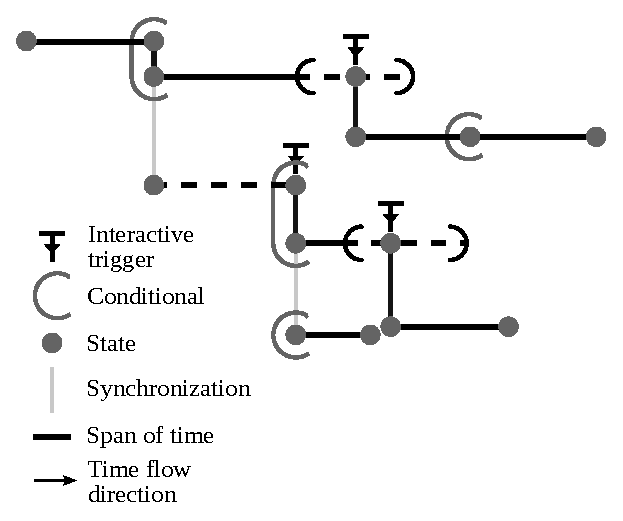
\includegraphics[width=0.35\textwidth]{images/iscore-example.eps}
  \caption{Part of an i-score scenario, showcasing the temporal syntax used. 
    A full horizontal line means that the time must not be interrupted, 
    while a dashed horizontal line means that the time of this time constraint can be interrupted to proceed 
  to the following parts of the score according to an external event.}
  \label{fig.iscore-example}
\end{figure}
    
\section{Definitions}
We call process an entity that consists in a state, an associated function $f$, any number of inputs and output ports, and an activation status.
$f$ has a single argument $t \in \mathbb{R^+}$.
The execution of $f$ may read any number of tokens from the inputs and write any number of tokens to the outputs.
    
We rely on two families of graphs for defining the execution of a program:
    
\begin{itemize}
  \item Synchronous dataflows between processes: input and output ports can be connected together to enforce data dependencies.
  \item Temporal graphs, based on the OSSIA formalism: $G_t(V_t, E_t)$ where $V_t$ is the set of time nodes and $E_t$ is the set of time constraints in a score. 
        For coherency, we call these graphs timeflows.
\end{itemize}

A program consists in the sequential and parallel execution of multiple processes, specified by a single dataflow, and at least one timeflow.
    
There may be more than a single timeflow: they are defined as processes themselves, which provides them with time information.
They have no input or output.
    
Each time constraint has an associated set of references to processes.
For each process in the dataflow, there is exactly one reference to this process in the set of all timeflows.
    
The execution of a program is synchronous and driven by a scheduler.
At each tick, the state of each temporal graph is updated with the following informations:
    
\begin{itemize}
  \item Which processes are currently activated.
  \item For how long these processes have been activated.
\end{itemize}

This is done according to the various events that occur and may trigger conditions and interaction points present in the temporal score.
    
Only activated processes may be called in a given tick.
    
% In a given tick, every active process will be executed. ?
%Event-driven vs time-driven vs sound-driven ; each node has a "driver" port which is the time or the sound. (Do like LV2: pass empty buffers). Pb: multi-rate ... voir méthode pour passer de multi-rate à single rate dans PLOP2006 et Signal Flow Graphs and Data Flow Graphs (3.2, 3.3), dans Handbook of Signal Processing (First Edition)
    
% Pour thèse: essayer de spécifier l'ensemble des cas possible / configuraitons d'activation de manière statique à partir d'un scénario donné, même si c'est exponentiel..

%\subsection{Why multiple graphs ?}
%\subsection{Hierarchy}
    
Throughout this paper, we will use the execution traces in fig.~\ref{fig.simple} and fig.~\ref{fig.simple-reversed} as running example. 
    
Finally, we will call developers the persons implementing dataflow-based software and users, authors, or composers the persons using dataflow-based software to implement their own music algorithms.
    
\begin{figure}
  \centering
  \begin{tikzpicture}[scale=0.5]
    \draw[line width=2pt] (0, 0) rectangle (5, 2);
    \draw[line width=2pt] (0 + 3, 0 - 2.5) rectangle (5 + 3, 2 - 2.5);
    		        
    \draw[line width=2pt] 
    (0, -3.75) -- 
    (0, -4) -- (3, -4) -- 
    (3, -3.75) --
    (3, -4) -- (5, -4) -- 
    (5, -3.75) -- 
    (5, -4) -- (8, -4) -- 
    (8, -3.75);
    		        
    \node (t1) at (1.45, -3.45) {\large $t_0$};
    \node (t2) at (4, -3.45) {\large $t_1$};
    \node (t3) at (6.5, -3.45) {\large $t_2$};
    		        
    \node (f1) at (2.5, 1) {\large $f_1$} ;
    \node (f2) at (5.5, -1.5) {\large $f_2$} ;
  \end{tikzpicture}
  \caption{A possible trace of execution for two processes}
  \label{fig.simple}
\end{figure}
	
\begin{figure}
  \centering
  \begin{tikzpicture}[scale=0.5]
    		        
    \draw[line width=2pt] (0 + 3, 0) rectangle (5 + 3, 2);
    \draw[line width=2pt] (0, 0 - 2.5) rectangle (5, 2 - 2.5);
    		                
    \draw[line width=2pt] 
    (0, -3.75) -- 
    (0, -4) -- (3, -4) -- 
    (3, -3.75) --
    (3, -4) -- (5, -4) -- 
    (5, -3.75) -- 
    (5, -4) -- (8, -4) -- 
    (8, -3.75);
    		        
    \node (t1) at (1.45, -3.45) {\large $t_0$};
    \node (t2) at (4, -3.45) {\large $t_1$};
    \node (t3) at (6.5, -3.45) {\large $t_2$};
    		        
    \node (f1) at (5.5, 1) {\large $f_1$} ;
    \node (f2) at (2.5, -1.5) {\large $f_2$} ;
  \end{tikzpicture}
  \caption{Another trace of execution with the same processes}
  \label{fig.simple-reversed}
\end{figure}


\begin{figure}
	\centering
	\begin{tikzpicture}[scale=0.5]
	 \node[draw, circle] (f1) at (0, 0) { $f_1$ };
	 \node[draw, circle] (f2) at (3, 0) { $f_2$ }
	    edge [<-] (f1);
	\end{tikzpicture}
	\caption{Another trace of execution with the same processes}
	\label{fig.simple-reversed}
\end{figure}
    
\section{Environment, implicit and explicit connections}
In the data flow paradigm, nodes are linked together through connections in their respective input and output ports.
    
This work extends it with a permanent external environment, that contains a mapping of key-value pairs.
Keys are specified with OSC-like\cite{Freed09featuresand} adresses: \lstinline|/foo/bar| and values can be any kind of data: numbers, strings, etc. 
The values of the environment may vary independently of the execution of the program: for instance elements of the environment may be changed asynchronously through the network, graphical widgets or physical controls.
    
We then have to provide a mean to use the values of this environment to the dataflow.
Thus, we extend the inputs and outputs ports with the following expliciteness semantic: 
    
\begin{itemize}
  \item An explicit port has been connected manually to another port.
        An input port may only read tokens from the output port it is connected to.
        	      
  \item An implicit port has not been connected to another port. 
        It may read and write to any number of adresses from the environment to perform its work.
        Every write done by a node is inserted in a sub-environment scoped to the duration of the tick.
\end{itemize}
    
During a tick, adresses have access to two sets of values: 
\begin{itemize}
  \item The values that were in the environment at the beginning of the tick.
  \item The values produced by previous implicit output ports in the dataflow.
        Section~\ref{sec.relationships} presents the various policies that nodes can leverage to 
        use these values.
\end{itemize}

Let $\mathrm{ticks}$ be the function that gives the number of ticks in an interval.+
For a given execution following fig.~\ref{fig.simple}, the evolution of such parameters may look like : 


\begin{table}
	\centering
	\begin{tabular}{c|ccc}
		Address & $t_0$ & $t_1$ & $t_2$ \\
		\midrule
		Global \lstinline|/a|  & $x$ & $x $ & \\
		Local \lstinline|/a|   & $\emptyset$ & & \\	
	\end{tabular}
	\caption{}
\end{table}

It is up to the implementor of nodes of the graph to choose whether a port can work: 
\begin{itemize}
  \item When connected explicitely,
  \item With the environment produced from previous nodes,
  \item With the global environment,
  \item With both of the previous.
\end{itemize} 

This mechanism allows for new behaviours during the creation of a dataflow program.
For instance, instead of accepting data from a single source, a port could specify an input pattern such as: \lstinline|/foo.*/bar/b[a-zA-Z]|, as proposed in the OSC specification.
% TODO pattern-matched addresses on the output: seems hard ? how to match it with a "pattern-matched" input port ??
%Inner data: reduces the possibilities of connection: everything has to be there (explicit)
	
%Outer data: have to care about overwriting (implicit)
%Implicit edges allow for features such as pattern-matching: one node outputs to random, unknown other inputs, or to the global state.
% For inputs to handle this, we have to provide them with a "can accept" function.
	
    
% TODO sample-precision of the activation / deactivation of a process / node
% TODO 
\section{Relationships}
\label{sec.relationships}
We are interested in the relationships between nodes of the dataflow graph when they produce compatible tokens, whether the production is specified implicitely or explicitely.
    
We propose five relationships : strict, glutton, delayed, mixed, and replaced. 
For some of these relationships, an ordering on the nodes is necessary. 
For this, a set of directed edges between nodes of the dataflow is used to provide this order.
Methods to set up these edges are discussed in section~\ref{sec.order}.
    
\subsection{Strict}
In a given tick, an execution of a sub-graph can only happen when all the nodes of the sub-graph are activated.
    
That is, if two nodes are compatible, the output of the first node can only go in the input of the second node when both are active.
    
For instance, take the case in fig.~\ref{fig.simple} where $f_1$ and $f_2$ both read from $/a$ and write to $/a$.
    
Let $t$ be the time of the tick and $e$ the global environment. 
We assume that $f_1, f_2$ always have access to this information.
    
We will get the following behaviours during each slice: 
\begin{itemize}
  \item During $t_0$: $\emptyset$.
  \item During $t_1$: $f_2 \circ f_1 $ or $f_1 \circ f_2$ depending on the node ordering.
  \item During $t_2$: $\emptyset$. 
\end{itemize}

The strict execution may happen explicitely or implicitely.
    
\subsection{Glutton}
An execution of a sub-graph can happen whenever any of the nodes of a sub-graph are executing. 
    
If we take the same case than previously, the behaviour is:
\begin{itemize}
  \item $t_0$: $f_1$.
  \item $t_1$: $f_2 \circ f_1$ or $f_1 \circ f_2$.
  \item $t_2$: $f_2$. 
\end{itemize}

The glutton execution may only happen when nodes are engaged in an implicit relationship.
    
\subsection{Delay}
A connection between an output and an input is delayed through bufferisation in a queue.
	
The delayed execution can behave in two ways:
\begin{itemize}
  \item Readers of the buffer always start from the same point : the beginning of the previous function in the callback chain.
  \item Readers of the buffer continue from the latest read position.
        In this case, the developer has to enforce that a single connection flowing from an output would be active at a given time, to prevent invalid reads .%Question: what happens in case of multiple read ?
\end{itemize}
	
%Note: this question has an answer in PLOP2006.
    
The delayed execution has be specified explicitely for the tokens to be bufferised.
It would be possible
    
If we have a delay connection from $f_1$ to $f_2$, the first call to $f_2$ will use the first value that was produced by $f_1$.
If the execution order happens to be reversed, such as in the case of fig.~\ref{fig.simple-reversed}, nothing will be read, and the execution will only happen during $t_1$.
	
\subsection{Parallelization and mixing}
All the sub-graphs are run with the same input environment. 
The resulting values put in the environment are undefined, but it is guaranteed that all values returned will have been set, which may trigger event handlers.
    
For audio or video streams however, a meaningful behaviour would be to mix all the outputs together.
    
Thus, we have to define summing operations for each of the data types supported.
    
We propose for instance the following operations: 
\begin{itemize}
  \item For simple parameters such as MIDI control changes or OSC messages: the latest value replaces the previous ones.
  \item For audio streams: two alternatives : the streams are mixed together, or the streams are put in additional channels.
  \item For MIDI notes: the notes are played together.
\end{itemize}

The parallelized execution may happen explicitely or implicitely.

\begin{itemize}
  \item $t_0$: $f_1$.
  \item $t_1$: $f_1$ and $f_2$ run in parallel, with the same value for $/a$.
  \item $t_2$: $f_2$. 
\end{itemize}
     
\subsection{Replacement}
All the nodes are run with the same input environment. 
The resulting values put in the environment are those of the latest node executing in the following dependent nodes.
    
Software authors may still have to execute the previous nodes if they happen to produce side-effects.
    
\begin{itemize}
  \item $t_0$: $f_1$.
  \item $t_1$: $f_1$ or $f_2$.
  \item $t_2$: $f_2$. 
\end{itemize}

The replaced execution may happen explicitely or implicitely.
    
\section{Specifying the relationships}
A remaining problem is the specification of the kind of relationship between two ports, and, more precisely, 
where this relationship should be specified.
    
We study the implication of bearing such annotations for each object in the dataflow.

\subsection{In the cables}
The most precise way to set-up dependency-related information would be in 
the cables connecting two ports. 
    
It is also the only way to set-up a delayed connection.
    
However, it would also be the most tedious for users if the patch changes often.
    
\subsection{In the ports}
\subsection{In the nodes}
\subsection{In the addresses}
No temporal behaviour possible
\subsection{Global behaviour}
No temporal behaviour possible
\subsection{Overall resolution}
Unspecified by default. 
    
Hierarchical: cable, port, node, address, global.
    
Default global behaviour: glutton.
    
  
\section{Default behaviours for orders}
\label{sec.order}
We study here the various behaviours possible to handle the dependency between nodes of the graph.
information provided provided in the timeflow can be leveraged to connect the nodes at runtime in a fashion 
that would make sense to composers \& authors.
    
By default, any non-ordered node would strive to be scheduled at the earliest possible time.
    
Connections between ports imply an ordering between nodes, hence we only consider the ordering between implicitely connected nodes of the dataflow.
    
\subsection{Manual ordering}
In this case, the author explicitely specifies an order by setting up an edge between two nodes. 
This is the slowest process, but which gives the most precise specification.
    
\subsection{Hierarchical}
We follow the hierarchical organization of the timeflows~: each time constraint has an ordered list of processes, and each time constraint is itself ordered relative to others in a given timeflow. 
This gives a natural order between processes.
    
\subsection{Temporal}
In this case, the temporal order in which objects are executed
will become the order of chaining in the dataflow.
    
    
\begin{figure}
  \begin{subfigure}{0.20\textwidth }    		    		
    \begin{itemize}
      \item $t_0$: $f_1$.
      \item $t_1$: $f_2 \circ f_1$.
      \item $t_2$: $f_2$. 
    \end{itemize}
    \caption{Glutton execution in the order of the fig.~\ref{fig.simple}}
  \end{subfigure}~
  \begin{subfigure}{0.20\textwidth}
    		    	
    \begin{itemize}
      \item $t_0$: $f_2$.
      \item $t_1$: $f_1 \circ f_2$.
      \item $t_2$: $f_1$. 
    \end{itemize}
    \caption{
    	Glutton execution in the case of fig.~\ref{fig.simple-reversed}}
  \end{subfigure}
  \caption{}
\end{figure}
    
\section{Evaluation algorithm}
- Split the tick in steps
- Each step, go to the next elements (follow the cables) and find all the nodes that can be currently called.
%We present here the evaluation algorithm that operates at each tick.
    
    
%Divide the time in abstract segment according to the activation graph; gives us a set of equations for each variable.
\section{Implementation}
\section{Conclusion}
Additional consideration: see PLOP 2006 article (multi-stream, etc), sample accuracy, etc
    
Explicit cables: optimization.

Generalization to not only a single variable of time, but any kind of driving parameters
\section{Acknowledgements}
\printbibliography 
\end{document}